\chapter{Fn: implementación}
\label{chap:fn-implementacion}

En este capítulo entraré en profundidad en la implementación de código del sistema, qué lenguaje de programación he usado y qué comunicaciones se realizan entre los distintos componentes que conforman \emph{Fn}.

Como se puede deducir de todos los apartados que hemos tocado para llegar aquí mi sistema usa Docker para preparar un contenedor de la función, Kubernetes para administrar las máquinas y lanzarlo, GRPC para comunicarse con el cliente de forma segura y RethinkDB como backend para almacenar datos. He elegido Go como lenguaje de programación principal aparte de diversos scripts en Bash, Makefile y otras herramientas parecidas.

Con el objetivo de conseguir un prototipo he diseñado la aplicación para funcionar en Minikube, el entorno de desarrollo sobre una máquina virtual de Kubernetes. Esto reduce evidentemente el rendimiento de forma que no podremos tomar mediciones de carga que sean significativas en ninguna decisión.

\section{Lenguaje de programación Go}

\subsection{¿Porqué Go?}

La elección de Go viene derivada de varios aspectos principales del lenguaje que favorecen la implementación de \emph{Fn}:
\begin{itemize}
    \item La implementación Go de GRPC es totalmente concurrente y mucho más avanzada que la del resto de lenguajes que soporta el framework.
    \item Es fácil implementar cualquier servicio web como el panel de control con una calidad digna de producción.
    \item Se pueden construir estructuras del lenguaje a partir del JSON que nos llega con unas simples anotaciones.
    \item Las facilidades que proporciona Go para la concurrencia nos permiten expresar los distintos componentes como actores independientes de cara a unos futuros microservicios. Además mantenemos los datos separados y evitamos elevar la dificultad de la aplicación al modificar ese estado interno.
    \item Construir un cliente REST para la API de Kubernetes no tiene complicación alguna usando la librería estándar del lenguaje.
    \item Genera un único binario que podemos incluir en el contenedor que se ejecutará en producción; no necesitamos intérpretes, ni servidores Tomcat, ni nada parecido.
    \item Concurrencia y paralelismo triviales, en el siguiente apartado lo amplio.
\end{itemize}

\subsection{Concurrencia y paralelismo}

Go introduce las herramientas que CSP\cite{Hoare:1978:CSP:359576.359585} (Communicating Sequential Processes) introduce como generalización de los \emph{guarded commands} de Dijkstra. Además introduce el concepto de gorutina para la concurrencia. Ambos forman la base de la facilidad y potencia que tiene ese lenguaje para este tipo de aplicaciones.

\subsubsection{Gorutinas}

Metafóricamente podríamos decir que son hebras, aunque se encuentran en un nivel de abstracción superior. Tienen un stack dividido que puede ir ampliándose a medida que surja la necesidad\cite{danielmorsing2014} en lugar de reservar de primeras memoria que nadie más puede usar como en el caso de las hebras.

Go posee un \emph{scheduler} que multiplexa las gorutinas en hebras\cite{morsing2013} dejando bloqueadas aquellas que hacen algún tipo de entrada/salida y usando las otras para seguir avanzando paralelamente trabajo con otras.

Es extremadamente fácil crear una nueva gorutina, simplemente hay que llamar a una función con \emph{go} delante:

\begin{minted}[baselinestretch=1.2]{go}
go foo()
\end{minted}

\subsubsection{CSP}

Este artículo define varias operaciones de comunicación\cite{robpike2010} entre distintos procesos para implementar un conjunto adecuado y válido para programación concurrente:
\begin{itemize}
    \item Mandar un valor a un proceso.
    \item Recibir un valor de un proceso.
    \item Ejecutar dos tareas en serie.
    \item Ejecutar dos tareas en paralelo (composición).
    \item Ejecutar una tarea repetidamente.
    \item \emph{Guarded command}, ejecutar un par de tareas dependiendo respectivamente de un par de condiciones; un \emph{if-else} pero paralelo.
\end{itemize}

Cualquier comunicación entre procesos actúa como punto de sincronización entre procesos.

Go recogió estos conceptos y los reflejó en forma de canales que permiten la comunicación entre gorutinas, y además mantienen una cola interna de mensajes pendientes de leer por si queremos que la escritura no sea bloqueante.

\begin{minted}[baselinestretch=1.2]{go}
foo := make(chan string)
go func() {
    str := <-foo
}()
foo <- "my string"
\end{minted}

\section{Fnctl}

\emph{Fnctl} es la interfaz de línea de comandos a nuestro sistema. Tiene un árbol de comandos y subcomandos a modo de \emph{git} o similares que permiten aplicar diferentes operaciones al clúster que administramos. Para comunicarse con el clúster establece una conexión GRPC con la API.

Uso una librería llamada Cobra\cite{cobra} para registrar estos comandos. Además se autogeneran descripciones y páginas de ayuda cuando ejecutamos el comando \emph{help} o añadimos el flag \emph{--help} a la llamada.

Para generar nuevas imágenes de contenedores cuando estamos desplegando una función se usa el propio cliente de Docker ejecutándolo por línea de comandos. En un futuro se prevé mover esta fase a un servidor de integración continua adecuada que no necesite colaboración del cliente y que sea más seguro.

\section{Docker registry}

El cluster ejecuta una instancia personal del registro de imágenes para subir los contenedores generados con las funciones que queremos ejecutar. El registro en sí mismo es un contenedor que ejecuto en el cluster siguiendo las instrucciones oficiales\cite{registrydeploy} para administrarlo.

Las imágenes están dipuestas para guardarse en la máquina de pruebas que tenemos. Ante una posible salida a producción habría que cambiar la definición del pod para que usara almacenamiento compartido de algún tipo, como NFS o un disco en la nube de Google Cloud.

\section{Fnapi}

El servicio para la API que administra el cluster. Se prepara dentro de un contenedor que se almacenará en el registro interno que tenemos. En un futuro despliegue a producción de la plataforma habría que elegir un registro centralizado como Docker Hub, Quay.io o Google Container Registry que almacene las versiones concretas en lugar de tener que configurar cada cluster con la imagen.

La aplicación implementa dos servidores: uno web para las estadísticas y el trigger HTTP y otro GRPC para la API en sí misma.

\section{Diagramas de secuencia de las operaciones}

\subsection{Listar funciones desde consola}

El listado de funciones reflejado en la figura \ref{fig:sec-list} implica que la herramienta debe contactar con el servidor de la API. Ésta a su vez saca la información directamente de la base de datos.

\begin{figure}[H]
    \centering
    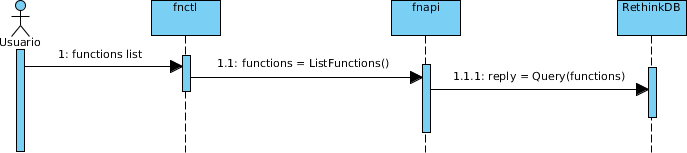
\includegraphics[width=\textwidth]{../images/secuencia/list-fnctl.png}
    \caption{Secuencia para listar funciones desde \emph{fnctl}}
    \label{fig:sec-list}
\end{figure}

\subsection{Listar funciones desde web}

Este caso es incluso más simple, porque es la API la que construye la plantilla de respuesta con lo que accede directamente a los datos almacenados en RethinkDB. Las interacciones las he reflejado sobre la figura \ref{fig:sec-list-web}.

\begin{figure}[H]
    \centering
    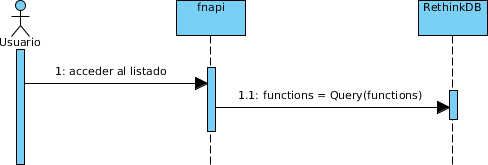
\includegraphics[width=\textwidth]{../images/secuencia/list-web.png}
    \caption{Secuencia para listar funciones desde la web}
    \label{fig:sec-list-web}
\end{figure}

\subsection{Despliegue de una nueva función}

El despliegue tiene un paso local y dos pasos remotos diferenciados. Primeramente construimos en nuestra máquina el contenedor con la aplicación. Fn se pone en contacto con el registro de contenedores para subir la imagen.

Cuando todo eso termina le pedimos a la API que cree las entradas correspondientes en la base de datos para la administración y en Kubernetes para iniciar/escalar el pod que ejecuta el contenedor.

\begin{figure}[H]
    \centering
    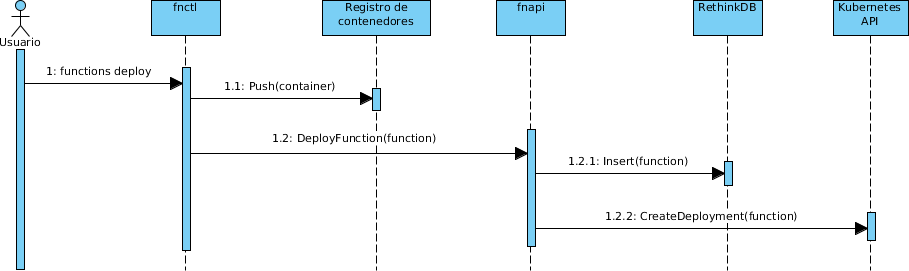
\includegraphics[width=\textwidth]{../images/secuencia/deploy.png}
    \caption{Secuencia para desplegar una nueva función}
\end{figure}

\subsection{Eliminar una función}

Un procedimiento simple que elimina los rastros de RethinkDB y la aplicación de Kubernetes para que se apaguen todos los contenedores.

\begin{figure}[H]
    \centering
    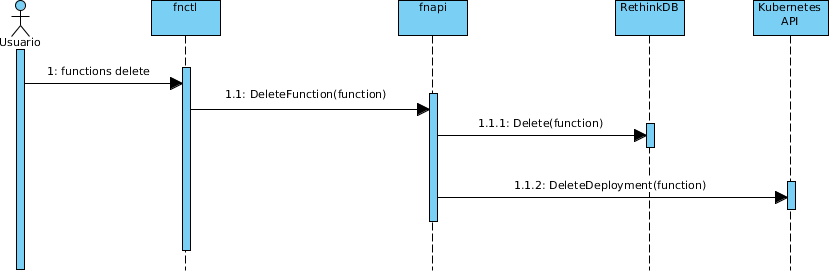
\includegraphics[width=\textwidth]{../images/secuencia/delete.png}
    \caption{Secuencia para eliminar una función}
\end{figure}

\subsection{Lanzar la función por HTTP}

En este gráfico se refleja gran parte de la arquitectura interna de la aplicación; así que procedo a enseñarlo y lo desglosaré justo debajo. Se recomienda usar el zoom o consultar el gráfico original directamente de la fuente online para evitar molestias.

\begin{figure}[H]
    \centering
    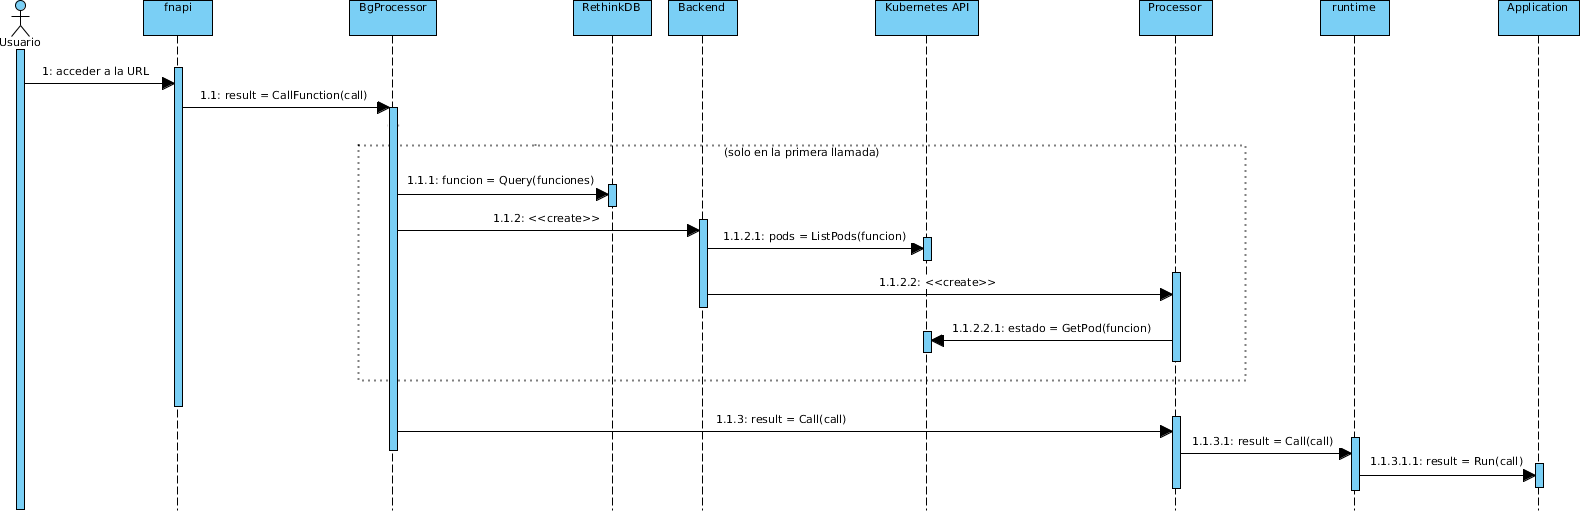
\includegraphics[width=\textwidth]{../images/secuencia/trigger-http.png}
    \caption{Secuencia para lanzar una función por HTTP}
\end{figure}

El sistema tiene varias rutinas de Go concurrentemente ejecutándose; a modo primitivo de microservicios comunicados por canales del lenguaje. La petición entra al sistema por el servicio web y entra en la cola del primer canal que lo lleva a una rutina en segundo plano llamada \emph{BgProcessor}. Esta rutina recoge llamadas de todo tipo y de todas las funciones y las procesa secuencialmente para meterlas en la cola del \emph{Backend} correspondiente.

Si es la primera llamada que se hace a una función debemos recuperar información de tiempo de ejecución desde la base de datos y crear un \emph{Backend} que controle los pods para el autoescalado de esa función.

El \emph{Backend} se encarga de monitorizar constantemente cuando aparecen y desaparecen pods consultando a la API de Kubernetes. Cuando aparece una nueva instancia se crea una rutina \emph{Processor} asociada que estará activa hasta que se elimine el pod. La rutina consulta Kubernetes para descubrir cuando se ha inicializado y cargado correctamente y cuando puede empezar a servir llamadas. Se mantendrá en ese estado de actividad hasta que la instancia deba ser sacrificada por recibir menos carga o por una eliminación explícita. El procedimiento para controlar los pods que se encienden o apagan lo veremos en la próxima subsección.

En resumen, todas las llamadas pasan por un \emph{BgProcessor} que las reparte a los backends correspondientes. Estos backends (uno por función) en proporción a la carga crean o destruyen instancias de la aplicación con un \emph{Processor} asociado a cada instancia. Este ejército de procesadores recogen llamadas del backend y las ejecutan en serie devolviendo el resultado al usuario.

\emph{Processor} en realidad habla un protocolo interno no documentado a propósito que en estos momentos es JSON sobre HTTP con un servidor autogenerado dentro del contenedor. Este runtime es el que se encarga de leer correctamente la petición y hacer la llamada a la aplicación del usuario que nos ha proporcionado al crear la función.

Indirectamente se observa que la API implementa un balanceo de carga muy primitivo entre las distintas instancias que conforman el servidor de la función.

\subsection{Autoescalado de instancias}

El propio \emph{Backend} se encarga periódicamente de comparar la carga que tiene pendiente de procesar con la cantidad de pods que hay activos en Kubernetes. Si el número es inferior, o demasiado superior al necesario tomará medidas creando o eliminando un pod respectivamente. Para ello escalará el deployment como fuera necesario para alcanzar el objetivo.

\begin{figure}[H]
    \centering
    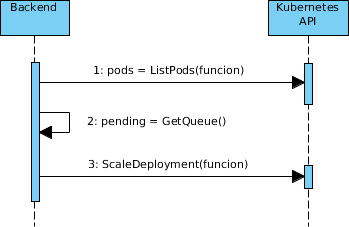
\includegraphics[width=\textwidth]{../images/secuencia/autoescalado.png}
    \caption{Secuencia para autoescalar las instancias de la función}
\end{figure}